%%%%%%%%%%%%%%%%%%%%%%%%%%% asme2e.tex %%%%%%%%%%%%%%%%%%%%%%%%%%%%%%%
% Template for producing hphrc-format articles using LaTeX
% Based on the asme2e template (http://iel.ucdavis.edu/code/ASME/)
% Modified by Antonio Attili
% In case of problem: antonio.attili@kaust.edu.sa
%%%%%%%%%%%%%%%%%%%%%%%%%%%%%%%%%%%%%%%%%%%%%%%%%%%%%%%%%%%%%%%%%%%%%%

%%%%%%%%%%%%%%%%%%%%%%%%%%%%%%%%%%%%%%%%%%%%%%
% To generate a pdf, compile either with pdflatex
% or with latex and
% dvips hphrc_template -Ppdf -t a4 -o
% followed by
% ps2pdf hphrc_template.ps
% (avoid using dvipdf that does not preserve the page layout on some systems)
%%%%%%%%%%%%%%%%%%%%%%%%%%%%%%%%%%%%%%%%%%%%%%

%%% use twocolumn and 10pt options with the hphrc format
\documentclass[twocolumn,10pt]{hphrc}
\usepackage{flushend}
\usepackage{graphicx}
\usepackage[authoryear,round]{natbib}

\title{Detailed numerical simulations of the autoignition-affected stabilization of laminar nonpremixed DME/air coflow flames}

%%%% In case you need to slightly adapt the horizontal spacing between authors (for more than 3 authors) uncomment the following command
%%%% and if necessary modify the factor
%\renewcommand{\expauthors}{1.1}

%%% first author
\author{Sili Deng, Peng Zhao, Michael E. Mueller, Chung K. Law
    \affiliation{
	Department of Mechanical and Aerospace Engineering\\
	Princeton University\\
    silideng@princeton.edu
    }	
}

%%% second author
%%% remove the following entry for single author papers
%%% add more entries for additional authors
%\author{Peng Zhao
%          \affiliation{Department of Mechanical and Aerospace Engineering\\
%	Princeton University\\
%	pzhao@princeton.edu
%    }
%}

%\author{Michael E. Mueller
%          \affiliation{Department of Mechanical and Aerospace Engineering\\
%	Princeton University\\
%	muellerm@princeton.edu
%    }
%}
%
%\author{Chung K. Law
%          \affiliation{Department of Mechanical and Aerospace Engineering\\
%	Princeton University\\
%	cklaw@princeton.edu
%    }
%}

\begin{document}

\maketitle   %Print title matter

% Set the font to 9pt.
\fontsize{9}{11}\selectfont

%%%%%%%%%%%%%%%%%%%%%%%%%%%%%%%%%%%%%%%%%%%%%%%%%%%%%%%%%%%%%%%%%%%%%%
\section*{ABSTRACT}

The structure and stabilization mechanism of laminar nonpremixed autoignitive DME/air coflow flames were investigated at elevated pressure and coflow temperatures, with constant jet and colfow velocities, using detailed numerical simulations.  The heat release rate and species profiles were examined for each case. Further investigation with Chemical Explosive Mode Analysis (CEMA) and Lagrangian Flamelet Analysis (LFA) were performed to identify the controlling chemistry and elucidate the dominant combustion mode and stabilization mechanism.  At $700$ to $900$ K, autoignition was observed to be the dominant stabilization mechanism, and NTC chemistry determines the stabilization point in mixture fraction space.  Moreover, the coupling between the autoignition process and premixed flame propagation results in a multibrachial structure.  Conversely, at $1100$ K, the kinematic balance between the premixed flame propagation velocity and the incoming flow velocity becomes the dominant stabilization mechanism, and the classical triple flame structure was observed.  Extended stabilization regimes, in terms of increasing boundary temperature, are therefore identified, including blow-off, purely kinetically stabilized, autoignition-propagation-coupled stabilized, purely kinematically stabilized, and burner stabilized regimes.

%%%%%%%%%%%%%%%%%%%%%%%%%%%%%%%%%%%%%%%%%%%%%%%%%%%%%%%%%%%%%%%%%%%%%%
\section*{COMPUTATIONAL DETAILS}

The flow configuration is an axisymmetric DME stream at $300$ K in a heated coflow of air ($700$, $800$, $900$, and $1100$ K) at $30$ atmospheres.  Uniform inlet velocities of $3.2$ m/s were specified for both fuel and air streams and kept the same for all the cases to establish lifted flames.

Dimethyl ether was chosen in this work, for it is a clean biofuel and one of the smallest hydrocarbons exhibiting the NTC behavior.  The present computations were conducted using a skeletal mechanism of $39$ species from ~\cite{bansal11}, including both low and high temperature oxidation pathways, which was reduced from the well validated detailed mechanism of~\cite{zhao08}.

%%%%%%%%%%%%%%%%%%%%%%%%%%%%%%%%%%%%%%%%%%%%%%%%%%%%%%%%%%%%%%%%%%%%%%
\section*{THERMAL STRUCTURE}

\begin{figure}[h]
  \centering
  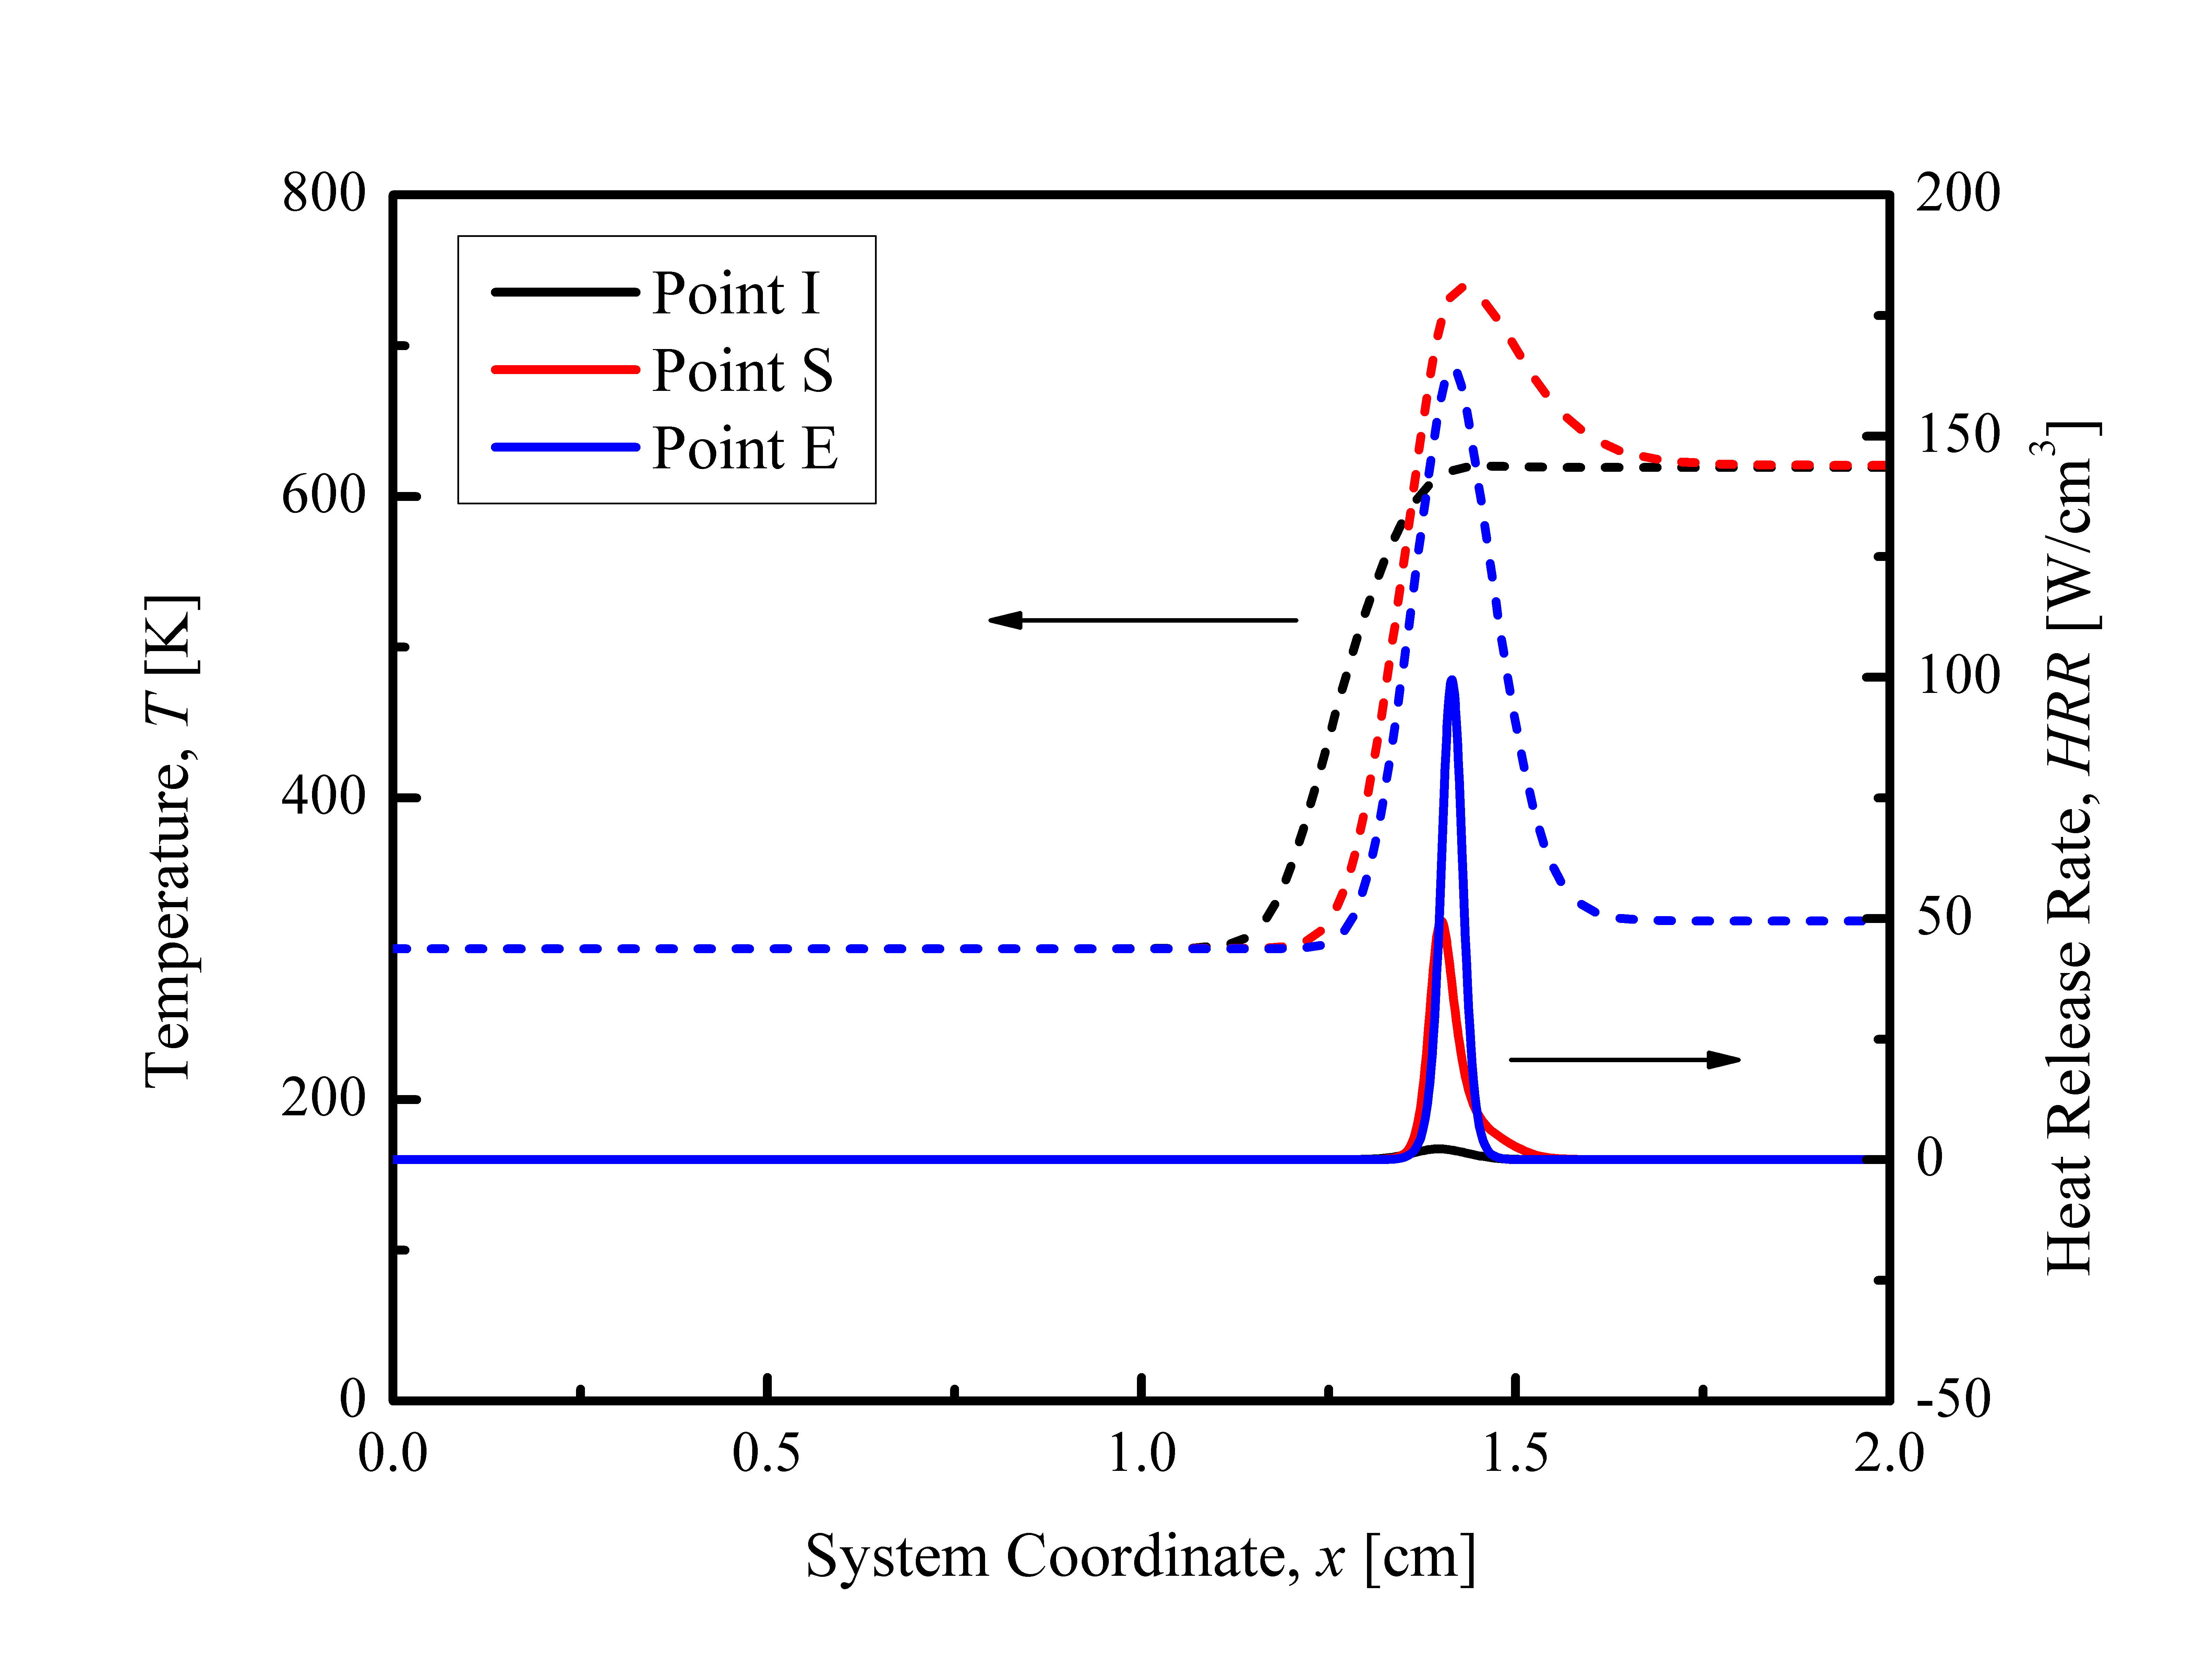
\includegraphics[width=3in]{HRR}
  \caption{Heat release rate [J/m$^3$-s] profiles.  The iso-contours of $Z_{\rm st}$, $Z = 0.2$, and $Z = 0.3$ are outlined from right to left in solid lines, respectively.  The CEMA sampling points at $800$ and $1100$ K are marked along the iso-contours.}
  \label{fig:HRR}
\end{figure}

To visualize the flame structures, the heat release rates profiles for the four cases are shown in Fig.~\ref{fig:HRR}.  Qualitatively, the most upstream point on the largest heat release contour (the leading point), colored by red, will be referred to as the stabilization point.

At $700$ K, a tribrachial thermal structure is observed, and the stabilization point locates around $Z = 0.15$, which is richer than the triple point.  Moreover, compared to the classical triple flame structure, the middle heat release rate branch, corresponding to the nonpremixed flame, is significantly weaker than the other two branches. 

At $800$ K, the stabilization point is not located on the triple flame structure any more.  Instead, it is located near $Z = 0.23$ and connects two trailing heat release branches, where a tribrachial flame structure is attached to the leaner branch of the bibrachial reacting front.

As the air boundary temperature increases to $900$ K, the stabilization point shifts back to $Z = 0.14$.  Moreover, a long trailing branch at richer mixture fraction is attached to the main triple flame, resulting in a tetrabrachial structure.  Compared with the structure shown in the $800$ K case, the main triple flame stabilizes further upstream, as it depends less on the radical accumulation ahead of the flame.  Therefore, it catches up with the reacting front at richer mixture fraction, and they merge as the tetrabrachial structure.

A further increase in the boundary temperature results in a structure that is very similar to the classical triple flame, except for the fact that there is also heat release ahead of the stabilization point at $Z = 0.13$.  Some of the multibrachial structures were also observed by~\cite{krisman14}, using different definitions for branches, and it was concluded that the autoignition chemistry could affect the flame structure and the stabilization mechanism.  


%%%%%%%%%%%%%%%%%%%%%%%%%%%%%%%%%%%%%%%%%%%%%%%%%%%%%%%%%%%%%%%%%%%%%%
\section*{COMPUTATIONAL DIAGNOSTICS AND ANALYSIS}

The above heat release rate profiles demonstrate the thermal structure of the reacting fronts at different boundary temperatures.  However, more detailed computational diagnostics and analysis are needed to further demonstrate the controlling chemistry and the stabilization mechanism.

%%%%%%%%%%%%%%%%%%%%%%%%%%%%%%%%%%%%%%%%%%%%%%%%%%%%%%%%%%%%%%%%%%%%%%
\subsection*{Chemical Explosive Mode Analysis}

Chemical Explosive Mode Analysis (CEMA) was conducted to identify the controlling chemistry in these complex reacting flows.  For each case, the local species concentrations and temperature were sampled along the $Z_{\rm st}$, $Z = 0.2$, and $Z = 0.3$ iso-contours, as marked in Fig.~\ref{fig:HRR}, and processed by CEMA to demonstrate the evolution of the dominant reactions.  

For the three lower coflow temperature cases, following the $Z_{\rm st}$ iso-contour, the dominant chain branching reaction shifts from H$_2$O$_2$ + M $\Longleftrightarrow$ OH + OH + M to H + O$_2$ $\Longleftrightarrow$ O + OH, indicating that the combustion mode shifts from autoignition to flame propagation.  The nature of the tribrachial structure (around $Z_{\rm st}$) at $700-900$ K is therefore identified: an autoignition assisted premixed flame front.

CEMA conducted along the $Z = 0.2$ iso-contour, which crosses the rich heat release front in the $800$ and $900$ K cases, shows different chemical mode evolution. The H$_2$O$_2$ chain branching reaction is always the dominant reaction.  Therefore, this heat release front is dominated by autoignition chemistry rather than flame chemistry and is considered as an autoignition front.

On the contrary, for the $1100$ K, the hydrogen peroxide chain branching reaction is not very important for all the sampled locations.  Since the hydrogen peroxide reaction is the crucial chain branching reaction for the autoignition process, it is concluded that the $1100$ K case is less affected by autoignition chemistry than the lower boundary temperature cases.  

%%%%%%%%%%%%%%%%%%%%%%%%%%%%%%%%%%%%%%%%%%%%%%%%%%%%%%%%%%%%%%%%%%%%%%
\subsection*{Lagrangian Flamelet Analysis}

To elucidate the role of autoignition for the current flow configuration, unsteady flamelet analysis was conducted to account for diffusion parallel to mixture fraction gradients, and comparisons with the two-dimensional computations can then demonstrate the dominant stabilization mechanism.

The $700-900$ K cases show good argeement between the flamelet profile with the time history of the two-dimensional computation, indicating that the thermal structure is stabilized by inhomogeneous autoignition.  

On the contrary, for the $1100$ K case, the ignition delay time computed with the one-dimensional flamelet assumption is significantly longer than the two-dimensional counterpart, indicating that autoignition is less important to the stabilization mechanism and that transport processes along the mixture fraction iso-contours must be important.

%%%%%%%%%%%%%%%%%%%%%%%%%%%%%%%%%%%%%%%%%%%%%%%%%%%%%%%%%%%%%%%%%%%%%%
\section*{STABILIZATION MECHANISM}
\begin{figure*}
  \centering
  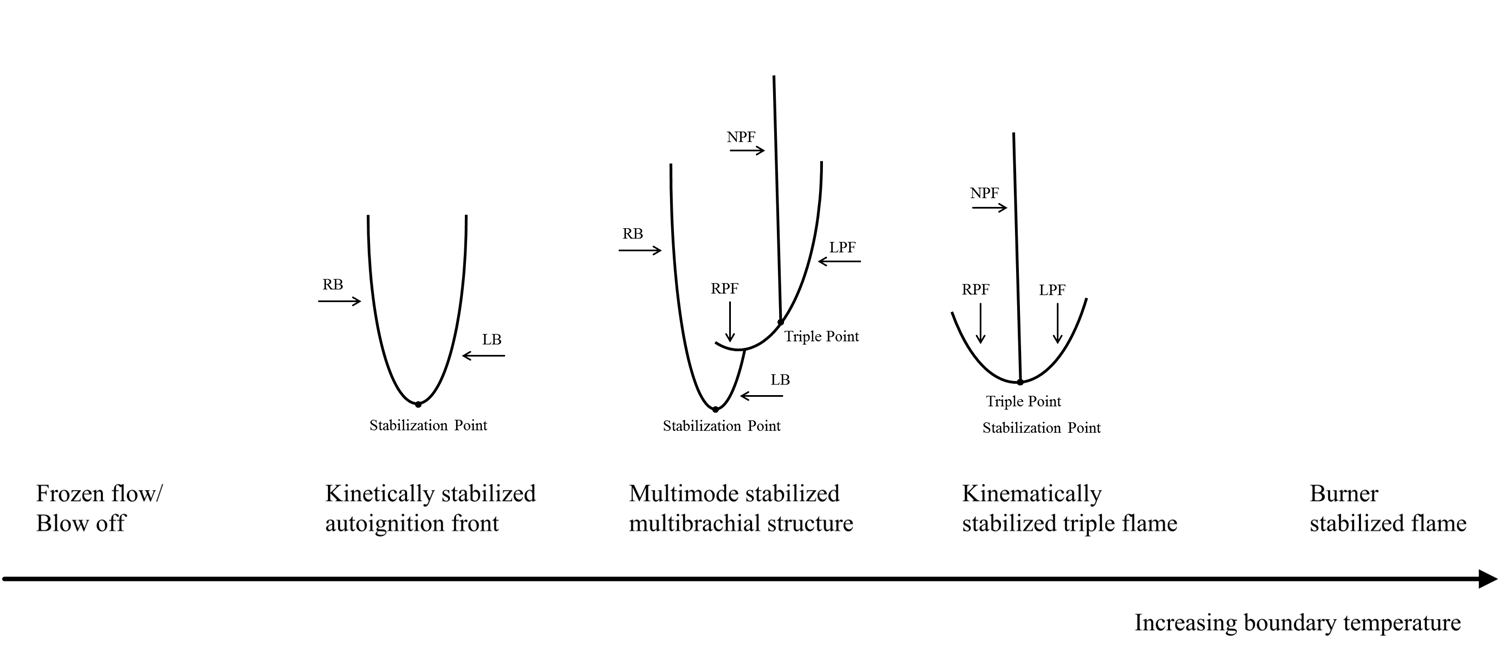
\includegraphics[width=5in]{regime}
  \caption{Extended regimes of the stabilization mechanism as coflow boundary temperature increases.}
  \label{fig:regime}
\end{figure*}

In the current study, two fundamental stabilization mechanisms are relevant: the \emph {kinetic} stabilization mechanism, due to the balance between the autoignition delay time and flow residence time, and the \emph {kinematic} stabilization mechanism, due to the balance between the premixed flame propagation velocity and the local flow velocity. 

In this stratified composition and temperature field, autoignition and flame propagation are coupled through thermal and radical interactions, for the accumulation of the upstream radicals and heat release from autoignition accelerate the flame propagation velocity.  The flame also transfers heat and radicals through back diffusion processes to the upstream, which could also facilitate autoignition.

Based on the understanding obtained from the current study, further extension of the stabilization regime can be made, as shown in Fig.~\ref{fig:regime}.  For sufficiently high inlet velocity, as the boundary temperature increases from the cold case, frozen flow is first achieved, where the mixture is nonautoignitive, and even the flame generated by an external ignition source will blow off.  When the mixture can be autoignited, the \emph {kinetically} stabilized autoignition front gradually transits to a \emph {kinematically} stabilized classical triple flame, where the premixed flame front propagation velocity balances the local incoming flow velocity.  The triple flame will eventually become attached when the boundary temperature is sufficiently high, and the flame speed is sufficiently fast.


%%%%%%%%%%%%%%%%%%%%%%%%%%%%%%%%%%%%%%%%%%%%%%%%%%%%%%%%%%%%%%%%%%%%%%
%\section*{REFERENCES}

\bibliographystyle{hphrc}
\bibliography{DME_KAUST}
% In this example, BibTeX is used
% For users not familiar with LaTeX, the bibliography can be typed in directly. In this case, comment the two lines above.
%%%%%%%%%%%%%%%%%%%%%%%%%%%%%%%%%%%%%%%%%%%%%%%%%%%%%%%%%%%%%%%%%%%%%%%
%\section*{SAMPLE REFERENCES}
%
%Kwon, O. K., and Pletcher, R. H., 1981, "Prediction of the Incompressible Flow Over a Rearward-Facing Step", Technical Report HTL-26, CFD-4, Iowa State Univ., Ames, IA.
%
%Lee, Y., Korpela, S. A., and Horne, R. N., 1982, "Structure of Multi-Cellular Natural Convection in a Tall Vertical Annulus," Proceedings, 7th International Heat Transfer Conference, U. Grigul et al., ed., Hemisphere Publishing Corp., Washington, D.C., Vol. 2, pp. 221-226.
%
%Sparrow, E. M., 1980a, "Fluid-to-Fluid Conjugate Heat Transfer for a Vertical Pipe - Internal Forced Convection and External Natural Convection", ASME Journal of Heat Transfer, Vol. 102, pp. 402-407.
%
%Sparrow, E. M., 1980b, "Forced-Convection Heat Transfer in a Duct Having Spanwise-Periodic Rectangular Protuberances", Numerical Heat Transfer, Vol. 3, pp. 149- 167.
%
%Tung, C. Y., 1982, Evaporative Heat Transfer in the Contact Line of a Mixture, Ph.D. Thesis, Rensselaer Polytechnic Institute, Troy, NY.

%%%%%%%%%%%%%%%%%%%%%%%%%%%%%%%%%%%%%%%%%%%%%%%%%%%%%%%%%%%%%%%%%%%%%%


\end{document}
